\chapter{Installation of Scientific Python}

\section{Introduction}

In this lab, you will install the software which we will be using in
phy40. This is an assignment, and will be graded.  You should submit a
text file containing a log of all the steps you took to install the
software on your computer.  Make this log as specific as possible, an
entry might be:
\begin{verbatim}
Downloaded windows installer from:
 https://repo.anaconda.com/miniconda/Miniconda3-latest-Windows-x86_64.exe
\end{verbatim}  
Keeping this log will also make it easier for you to get help if you
have problems.

If you run into problems, do some research on a web search tool
(Google, for example) to become better informed and to see if you can
overcome the problem on your own before asking for help.  This is an
important technique in getting help with technical problems that will
serve you well even outside of this class.  You will find it more easy
to get useful technical help, from the sort of people most capable of
offering it, when it is clear from your question that you are informed
and have already tried all of the obvious things.  If you are still
stuck after trying to solve the problem for yourself, then contact
your TA or instructor with specific technical details about what is
failing, and include your installation log.

If you do find a problem with these instructions or manage to overcome
a technical problem yourself, make sure to note it in your log and
inform your TA, in case it is helpful for other students.

\section{Installing Miniconda3}

We will be using Miniconda3 based on Python 3.7 for data analysis
using Jupyter notebooks.  Miniconda is a lightweight package which we
can use to install all of the remaining analysis software we will need
in a consistent manner across all different operating systems.

Determine which OS type and version you have on the desktop or laptop
computer that you will be using for your coursework.  The software
here will work under Windows, Linux, or macOS.  It should also work on
all Chromebooks released since 2019, and some earlier Chromebooks.
You should also check whether you have a 32-bit or 64-bit OS (you can
find instructions for how to determine this for your particular OS
version with a Google search.)  Most desktop or laptop computers built
in the last ten years are 64-bit.

If you are using Linux or macOS, then from within a terminal type:
\begin{lstlisting}{language=csh}
 echo $SHELL
\end{lstlisting}
to determine the shell you are using (typically "bash" these days).
Record all of this information in your installation log file.

Once you have determined your OS type and version, follow the
instructions below approprate to your operating system.

\subsection{Installing under Windows}

If you have already installed a version of conda (e.g. Anaconda or
Miniconda) then you do not need to re-install it.  Instead, find the
the Anaconda Prompt in the Application menu and run it.

If you need to install Miniconda3, then download and run the
appropriate installer from:
\begin{verbatim}
https://docs.conda.io/en/latest/miniconda.html#
\end{verbatim}
If prompted, you should choose to:
\begin{itemize}
 \item Accept the license / terms of use.
 \item Install for just the current user, not all users.
\end{itemize}
 Once installed, check that you can run the "Anaconda Prompt". From
the prompt, check that you can run:
\begin{lstlisting}{language=csh}
  conda --version
\end{lstlisting}
and note the output in your installation log.  Then proceed to
Section~\ref{sec:env}.

\subsection{Installing on a Chromebook}

You will need to activate Linux on your Chromebook, according to the instructions here:

\begin{verbatim}
https://www.codecademy.com/articles/programming-locally-on-chromebook
\end{verbatim}

Then follow the insturctions for installing under Linux.  If your
Chromebook predates 2019 and does not support Linux, contact your
instructor for alternative arrangements.

\subsection{Installing Miniconda3 under Linux or macOS}

If you believe you already already have a version of conda installed
(such as miniconda or ananconda) , check by running
\begin{lstlisting}{language=csh}
   conda --version
\end{lstlisting}
If you see something like:
\begin{lstlisting}{language=csh}
  conda 4.9.2
\end{lstlisting}
as output (even if the version is different) then you do indeed already have conda
installed, with the base environment activated, and you can skip ahead to
Section~\ref{sec:env}.  If instead you get a message like:
\begin{lstlisting}{language=csh}
   conda: command not found
\end{lstlisting}
then the easiest solution is to simply proceed with these instructions.

To install Miniconda, download the appropriate installer for your OS
here:
\begin{verbatim}
  https://docs.conda.io/en/latest/miniconda.html\#
\end{verbatim}
For macOS, you can choose between a "package" or "bash" version. I
find it easier to follow the bash version, but the package version
will work too. I recommend you make the following choices if prompted:
\begin{itemize}
\item Accept the license / terms of use.
\item Do not install for all users, but just one the current user.
\item Do allow the installer to issue ``conda init''.
\end{itemize}
During the installation, take note of the install location in your log.

After installation with these settings, conda will automatically
activate the ``base'' conda environment.  If this annoys you, as it
does me, or interferes with other software you are using, you can turn
off this agressive behavior with:
\begin{lstlisting}{language=csh}
   conda config --set auto_activate_base false
\end{lstlisting}

Confirm that you have successfully installed conda by typing
\begin{lstlisting}{language=csh}
   conda --version
\end{lstlisting}
Record the output in your installation log, and proceed to Section~\ref{sec:env}.

\section{Installing the Physics 40 Conda Environment}
\label{sec:env}

Make sure your conda is fully up to date with:
\begin{lstlisting}{language=csh}
  conda update conda
\end{lstlisting}
Then follow the prompts, e.g. selecting "y" as needed to update any out-of-date packages.

We'll be using a conda environment specifically for phy40 to avoid
conflicts with any other projects on your computer, and to ensure that
we all have the same software installed.  To create our environment:
\begin{lstlisting}{language=csh}
  conda create -n phy40 python=3.9 numpy scipy matplotlib ipython jupyter
\end{lstlisting}
  
\section{Starting a Jupyter notebook}

This course will make extensive use of the Jupyter Notebook interface
to Scientific Python, which is well suited to academic work (including
independent research) because it combines code with output in
digestable chunks.  Even when the end product is a polished peice of
software, much of the initial code development can be done in the interactive
session that Jupyter Notebooks provide.  

\begin{figure}[htbp]
\begin{center}
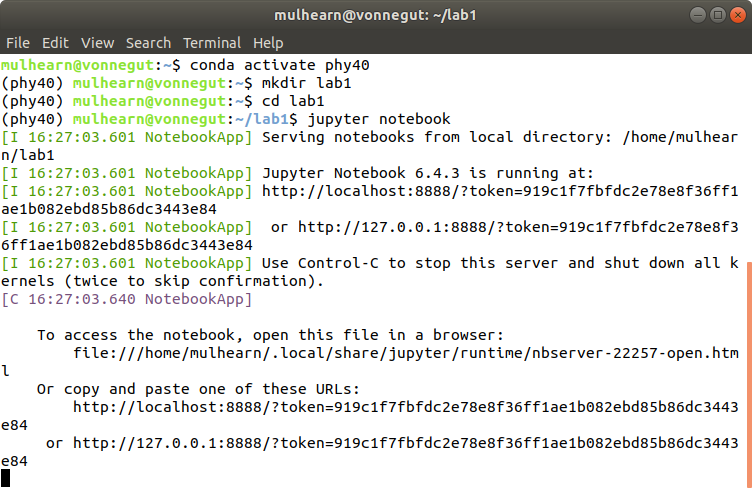
\includegraphics[width=0.65\textwidth]{figs/install/jupyter_startup.png} 
\caption{Example starting Jupyter Notebook from the Linux command line.  In Windows, you will need to open the Anaconda Prompt instead of a terminal.}
\label{fig:jupyterstartup}
\end{center}
\end{figure}

\begin{figure}[htbp]
\begin{center}
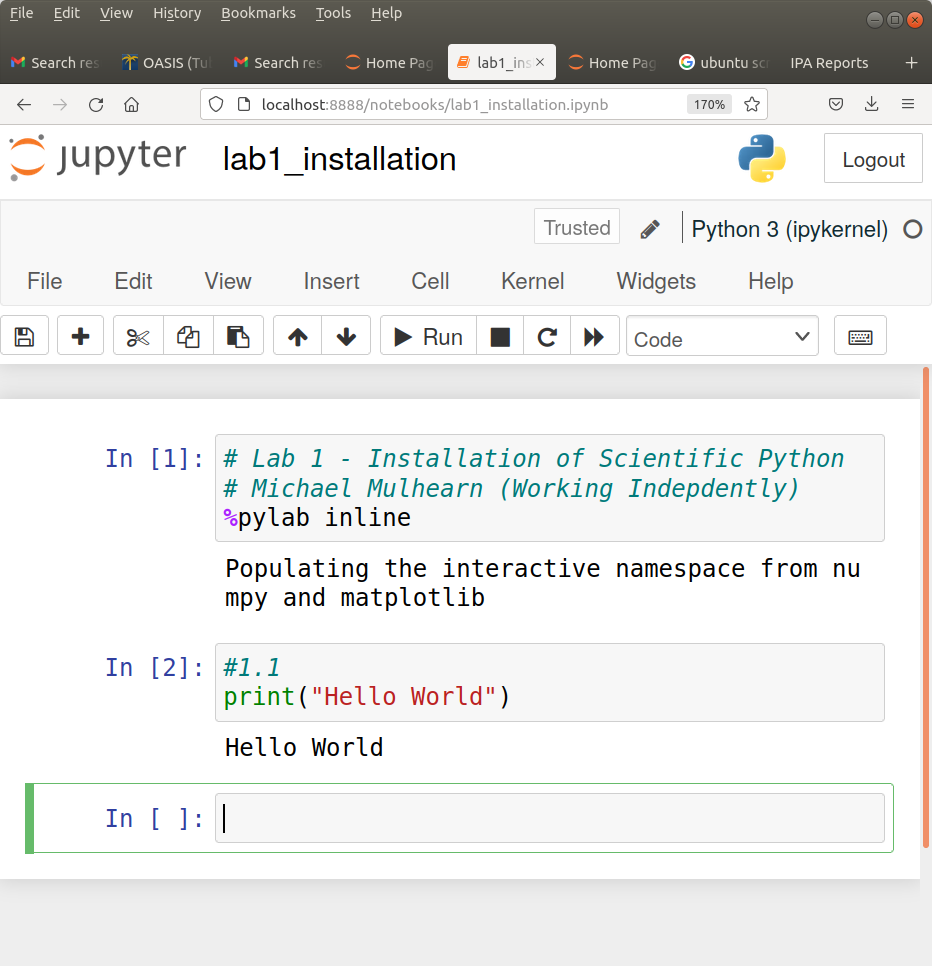
\includegraphics[width=0.65\textwidth]{figs/install/jupyter_window.png} 
\caption{The Hello World example Jupyter Notebook.}
\label{fig:jupyterwindow}
\end{center}
\end{figure}

\begin{figure}[htbp]
\begin{center}
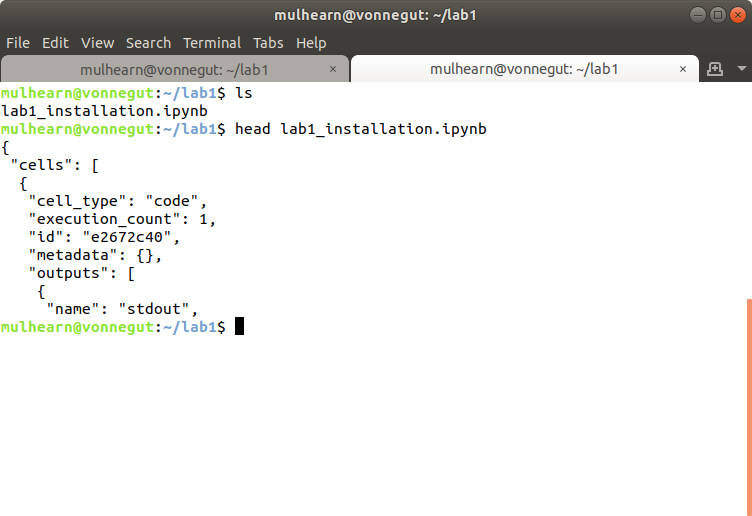
\includegraphics[width=0.65\textwidth]{figs/install/jupyter_saved.png} 
\caption{Example showing the saved Jupyter notebook.  Notice that notebook file (ipynb) is not human readable on its own: it requires the Jupyter software to render it in a human readable form.}
\label{fig:jupytersaved}
\end{center}
\end{figure}

To activate the phy40 environment type:
\begin{lstlisting}{language=csh}
  conda activate phy40
\end{lstlisting}
When you are done with Phy 40 for the day you can deactivate this
environment (later) with:
\begin{lstlisting}
  conda deactivate
\end{lstlisting}
Launch jupyter notebook with:
\begin{lstlisting}
  jupyter notebook
\end{lstlisting}
This should start the Jupyter Notebook server and open a client in your web browser.
An example starting a Jupyter Notebook from Linux is shown in Fig.~\ref{fig:jupyterstartup}.

You should create one Jupyter Notebook per lab assignment, by choosing
the New (Python 3) option in your client.  Change the name of your
notebook to something that clearly identifies the lab.  Start each lab
with comments (starting with ``\#'' symbol) indicating the title of
the lab, then your name followed by your lab partners.  See the first
cell of Fig.~\ref{fig:jupyterwindow} for an example.  This first cell
is also a good place to issue the ipython ``magic function'':
\begin{verbatim}
%pylab inline
\end{verbatim}
which will setup the notebook for inline plots and load the numpy and matplotlib libraries for you.

Each assignment will consist of a number of steps, clearly numbered like this one, your first step:\\

\plot Print ``hello world'' using the python print command.\\

\noindent
To keep your notebook clear, label cells (such as this one) with a
comment for the assignment step number, as in the second cell of
Fig.~\ref{fig:jupyterwindow}.  You only need to label one cell if the
assignment is fullfilled across several cells.

Jupyter Notebook checkpoints your work automatically.  You should be
able to see your notebook saved in the working directory where you
started, as in Fig.~\ref{fig:jupytersaved}.  Notice that while the
notebook file is ASCII text, it is not a human readable format.  The
Jupyter software is needed to render the notebook in a human readable
way.  To make your grader's life easier, you will be submitting PDF
versions of your notebook, once all of the tasks are completed and the
output is visible.  There are several ways to make a PDF file from
your notebook, but the most reliable is to use the ``Print Preview''
option to view the notebook as a PDF file within your browser, then
use the print feature of your browser to print the page as a PDF file.
Try this now, and make sure you can create a legible PDF file, but do
not submit it to the course site, as you still have more to do.
Always keep your python notebook file (ipynb) even after you submit
the assignment.  If you have problems, you can reproduce a PDF file
from the notebook file, but it is tedious to reproduce your notebook
from PDF.  If you have problems producing the PDF file, you can submit
the ``ipynb'' file as a temporary work-around, but work with your TA
to sort out the problem as quickly as possible.

\section{Submitting your assignment}

Before submitting, take some time to clean up your assignments to
remove anything superfluous and place the exercises in the correct
order.  You can also add comments as needed to make your work clear.
You can use the Cell $\to$ All Output $\to$ Clear and Cell $\to$ Run
All commands to make sure that all your output is up to date with the
cell source.

When you are satisfied with your work, print the PDF file as described
earlier and submit it to the course website.









